% !TEX program = lualatex
\documentclass[10pt,a4paper]{article}

% ----------------------------- ГЕОМЕТРИЯ ------------------------------------
\usepackage[a4paper,left=1.75cm,right=1.55cm,top=1.9cm,bottom=1.7cm,
            headheight=12pt,headsep=6pt,footskip=1.0cm]{geometry}

% ------------------------------- ШРИФТЫ -------------------------------------
\usepackage{fontspec}
\usepackage[russian]{babel}

\setmainfont{Inter}[Path=fonts/, Extension=.ttf,
  UprightFont=Inter-Regular,
  BoldFont=Inter-SemiBold,
  ItalicFont=Inter-Italic,
  BoldItalicFont=Inter-SemiBoldItalic]
\newfontfamily\mediumfont{Inter}[Path=fonts/, Extension=.ttf,
  UprightFont=Inter-Medium]

% ------------------------------ ПАКЕТЫ --------------------------------------
\usepackage{amsmath,amssymb}
\usepackage{booktabs}
\usepackage{tabularx}
\usepackage{array}
\usepackage{graphicx}
\usepackage{xcolor}
\usepackage{caption}
\usepackage{enumitem}
\usepackage{microtype}
\usepackage{eso-pic}
\usepackage{fancyhdr}
\usepackage[most]{tcolorbox}
\usepackage[hidelinks]{hyperref}

% ------------------------------- ЦВЕТА --------------------------------------
\definecolor{ink}{HTML}{111417}
\definecolor{muted}{HTML}{959595}
\definecolor{accent}{HTML}{173A63}
\definecolor{linkblue}{HTML}{5F86DC}
\definecolor{rule}{HTML}{D9E2EC}
\definecolor{boxbg}{HTML}{F7F9FC}

\hypersetup{
  colorlinks=true,
  linkcolor=linkblue,
  urlcolor=linkblue,
  pdftitle={Нижняя оценка взаимной информации: MINE},
  pdfauthor={Борисов Никита}
}

% ---------------------------- ОФОРМЛЕНИЕ ТЕКСТА -----------------------------
\linespread{1.5}
\setlength{\parindent}{0pt}
\setlength{\parskip}{0.45em}
\setlength{\emergencystretch}{2.5em}
\renewcommand{\arraystretch}{1.15}

\captionsetup{font=small, labelfont={bf}, skip=5pt}

% --------------------------- ВОДЯНОЙ ЗНАК (ЛОГО) ----------------------------
\newcommand{\logo}{%
  \put(\LenToUnit{\dimexpr\paperwidth-1.55cm-1.15cm\relax},%
       \LenToUnit{-1.82cm}){%
    
\includegraphics[width=1.15cm]{figs/logo.png}}}
\AddToShipoutPictureBG{\AtPageUpperLeft{\logo}}

% ------------------------------ КОЛОНТИТУЛ ----------------------------------
\pagestyle{fancy}
\fancyhf{}
\fancyhead[L]{\fontsize{7.5}{9}\selectfont\color{muted}Вариационные оценки · MINE}
\fancyfoot[C]{\fontsize{8}{10}\selectfont\color{muted}\thepage}
\renewcommand{\headrulewidth}{0pt}
\renewcommand{\footrulewidth}{0pt}

% ------------------------------- МАКРОСЫ ------------------------------------
\newcommand{\lesson}[2]{%
  \par\addvspace{16pt plus 4pt}%
  \phantomsection\hypertarget{sec:#1}{}%
  \noindent{\mediumfont\fontsize{12.5}{15}\selectfont
    \MakeUppercase{#1.\enspace#2}}\par
  \addvspace{5pt}}
\newcommand{\sublesson}[2]{%
  \par\addvspace{10pt}%
  \noindent{\bfseries\fontsize{10.8}{13}\selectfont #1\enspace#2}\par
  \addvspace{3pt}}
\newcommand{\heading}[1]{%
  \par\addvspace{16pt plus 4pt}%
  \noindent{\mediumfont\fontsize{12.5}{15}\selectfont\MakeUppercase{#1}}\par
  \addvspace{5pt}}

% ------------------------------- ТИТУЛ --------------------------------------
\newcommand{\titleblock}{%
  \par\addvspace{4pt}%
  {\fontsize{20}{23.5}\selectfont\bfseries Нижняя оценка взаимной информации:\\ метод MINE}\par
  \addvspace{7pt}%
  {\fontsize{8.5}{10.5}\selectfont\color{muted}%
   Борисов Никита\enspace·\enspace 2 курс, трек ML\enspace·\enspace
   n.borisov@edu.centraluniversity.ru\enspace·\enspace Москва, 2026}\par
  \addvspace{14pt}}

% ---------- неплавающие объекты: ровно на своём месте в тексте --------------
\newcommand{\fig}[4]{% {ширина}{файл}{подпись}{метка}
  \par\addvspace{4pt}%
  \noindent\begin{minipage}{\linewidth}\centering
    \includegraphics[width=#1\linewidth]{#2}\par
    \captionof{figure}{#3}\label{#4}
  \end{minipage}\par\addvspace{6pt}}

\begin{document}

\thispagestyle{fancy}
\titleblock

Взаимная информация (ВИ) измеряет статистическую зависимость двух случайных
величин и, в отличие от корреляции, видит и нелинейные связи: для $Y=X^2$
корреляция равна нулю, а информация о связи — нет. В работе рассмотрены три
способа оценить ВИ по выборке: гистограммный (\textsc{Binning}), $k$NN-оценщик
(\textsc{KSG}) и нейросетевой \textsc{MINE}. Основным выбран \textsc{MINE} —
он даёт \emph{нижнюю} оценку и позволяет максимизировать ВИ; его «зеркало»,
верхняя оценка \textsc{CLUB}, нужна для минимизации и в этой части не
рассматривается.

{\fontsize{8}{10}\selectfont\color{muted}Краткий план}\par\addvspace{2pt}
\begin{itemize}[leftmargin=2.2em, label={\color{linkblue}\small$\bullet$}, itemsep=1pt]
  \item \hyperlink{sec:1}{Метрики: что такое взаимная информация}
  \item \hyperlink{sec:2}{Постановка: гауссовская модель с известным ответом}
  \item \hyperlink{sec:3}{Методы: Binning, KSG, MINE}
  \item \hyperlink{sec:4}{Бейзлайны на малой размерности}
  \item \hyperlink{sec:5}{MINE: сравнение и валидация}
\end{itemize}

% ============================================================================
\lesson{1}{Метрики}

Взаимная информация — это дивергенция Кульбака--Лейблера между совместным
распределением и произведением маргинальных:
\begin{equation}\label{eq:mi}
  I(X;Y) = D_{\mathrm{KL}}\big(p(x,y)\,\|\,p(x)p(y)\big)
         = \mathbb{E}_{p(x,y)}\!\left[\log\frac{p(x,y)}{p(x)p(y)}\right].
\end{equation}
Свойства, на которых держится вся дальнейшая проверка: $I\ge 0$; $I=0$
тогда и только тогда, когда $X$ и $Y$ независимы; $I$ симметрична; и $I$ не
меняется при обратимых преобразованиях данных — $I(f(X);g(Y))=I(X;Y)$ для
биекций $f,g$, потому что якобианы сокращаются в отношении плотностей.

Точный расчёт \eqref{eq:mi} требует плотностей, которых на практике нет: есть
только выборка пар $\{(x_i,y_i)\}_{i=1}^N$. Поэтому ВИ оценивают, а
«правильность» оценки проверяют по направлению границы: нижняя оценка должна
лежать ниже истины, верхняя — выше.

% ============================================================================
\lesson{2}{Постановка задачи}

Проверка идёт на синтетике, где истинный ответ известен. Берём
$(X,Y)$ совместно гауссовскими размерности $d$:
\begin{equation}\label{eq:model}
  x \sim \mathcal{N}(0,I_d),\qquad
  y = \rho\,x + \sqrt{1-\rho^2}\,\varepsilon,\qquad
  \varepsilon \sim \mathcal{N}(0,I_d),
\end{equation}
где $\varepsilon$ не зависит от $x$. Тогда
$\operatorname{corr}(x_i,y_j)=\delta_{ij}\rho$: каждая координата $y_i$
связана только со «своей» $x_i$ с одним и тем же коэффициентом $\rho$, а
между разными координатами корреляция нулевая. Для этой модели
\begin{equation}\label{eq:true}
  I(X;Y) = -\frac{d}{2}\,\log\!\big(1-\rho^2\big),
\end{equation}
и при $\rho=0$ получаем $I=0$ (независимость), а при $\rho\to1$ — расходимость.

В основной серии $d=10$, а сетка — 30 точек $\rho\in[0.1,\,0.99]$; она даёт
$I\approx 0.05\ldots19.6$ нат, причём заявленный в задании диапазон 2--10 нат
покрывается её частью ($\rho\approx0.59\ldots0.93$). Качество оценки измеряем
направлением границы ($\hat I\le I$ для \textsc{MINE}), смещением
$\hat I-I$ и разбросом по сидам.

% ============================================================================
\lesson{3}{Методы}

\sublesson{3.1}{Binning}
Идея — самая прямая: разложить обе величины по бинам и посчитать частоты.
Бины удобно брать по квантилям, чтобы клетки получались равновероятными;
тогда по нормированной совместной гистограмме получаются оценки
$\hat p_{xy}$, $\hat p_x$, $\hat p_y$, и остаётся подставить их в
определение \eqref{eq:mi}:
\begin{equation}\label{eq:bin}
  \hat I_{\text{bin}} = \sum_{i,j}\hat p_{xy}[i,j]\,
  \log\frac{\hat p_{xy}[i,j]}{\hat p_x[i]\,\hat p_y[j]}.
\end{equation}
Метод не требует обучения и легко интерпретируется, но у него две беды:
смещение (при малом $N$ и многих бинах он завышает, при малом числе бинов —
занижает) и проклятие размерности: клеток $B^{2d}$, поэтому он применим
только при малых $d$.

\sublesson{3.2}{KSG}
\textsc{KSG} не строит сетку, а адаптируется к локальной плотности: для каждой
точки ищутся $k$ ближайших соседей, и плотность оценивается по расстояниям до
них (оценка энтропии Козаченко--Леоненко). Оценщик ВИ — это комбинация трёх
таких оценок — совместной и двух маргинальных; трюк в том, что один и тот же
радиус $\varepsilon$ берётся из совместного пространства и переиспользуется в
маргиналах, поэтому расстояния сокращаются, и остаются только счётчики соседей:
\begin{equation}\label{eq:ksg}
  \hat I_{\text{KSG}} = \psi(k) + \psi(N) -
  \frac1N\sum_i\Big[\psi\big(n_x(i)+1\big) + \psi\big(n_y(i)+1\big)\Big],
\end{equation}
где $n_x(i)$ — число точек в $x$-шаре радиуса $\varepsilon_i$, $n_y(i)$ — то
же по $y$, а $\psi$ — дигамма-функция, возникающая из $k$NN-оценки энтропии.
Вывод и свойства — в оригинальной работе~[2]; для дальнейшего важно
только, что оценка строится по счётчикам соседей, не требует плотностей и не
имеет бинов.

\fig{0.40}{figs/ksg_schematic.png}{Устройство \textsc{KSG}: радиус
$\varepsilon$ до $k$-го соседа в совместном пространстве и счётчики $n_x$,
$n_y$ в маргиналах.}{fig:ksg}

\sublesson{3.3}{MINE}
\textsc{MINE} опирается на двойственное представление Донскера--Варадхана:
\begin{equation}\label{eq:dv}
  D_{\mathrm{KL}}(P\|Q) = \sup_{T}\Big\{
    \mathbb{E}_{P}[T] - \log\mathbb{E}_{Q}\big[e^{T}\big]\Big\}.
\end{equation}
При $P=p(x,y)$, $Q=p(x)p(y)$ и критике $T_\theta$, который параметризует сеть:
\begin{equation}\label{eq:mine}
  I(X;Y)\ \ge\ \hat I_{\text{MINE}}(\theta)
  = \mathbb{E}_{p(x,y)}[T_\theta] - \log\mathbb{E}_{p(x)p(y)}\big[e^{T_\theta}\big].
\end{equation}
Равенство достигается при $T^*(x,y)=\log\frac{p(x,y)}{p(x)p(y)}$ — сеть учит
логарифм отношения плотностей, не зная самих плотностей. На батче:
\begin{equation}\label{eq:batch}
  \hat I_{\text{MINE}} = \frac1N\sum_{i=1}^{N}T_\theta(x_i,y_i)
  - \log\Big(\frac1N\sum_{i=1}^{N} e^{T_\theta(x_i,\,y_{\pi(i)})}\Big),
\end{equation}
где положительные пары $(x_i,y_i)$ берутся из совместного распределения, а
отрицательные получаются перемешиванием $y$ в батче (случайная перестановка
индексов): перемешанная пара распределена как $p(x)p(y)$. Второй член
считается через \texttt{logsumexp} (иначе $e^{T}$ переполняет float), а среднее
$\mathbb{E}_Q[e^{T}]$ оценивается по мини-батчу с экспоненциальным скользящим
средним — это убирает смещение градиента $\log\mathbb{E}_Q[e^T]$.

Интуиция. Оценка $\hat I_{\text{MINE}}$ — это ещё и лосс из двух частей:
(1) скор положительных пар — модель учится «выуживать» максимум информации из
настоящих пар; (2) минус скор отрицательных пар — та же модель не должна
выдавать информации о перемешанных парах, ведь связи между ними нет. Поэтому
при независимых величинах скор получается нулевым: перемешанные пары дают
такой же скор, как настоящие. Решаем задачу \emph{градиентного подъёма},
поскольку \textsc{MINE} — нижняя оценка на $I$ (в коде лосс берётся со знаком
минус, так как оптимизатор минимизирует).

Почему критик должен быть квадратичным. В гауссовской модели
\begin{equation}\label{eq:tstar}
  T^*(x,y)=\frac{\rho}{1-\rho^2}\,(x\cdot y)
  -\frac{\rho^2}{2(1-\rho^2)}\big(\|x\|^2+\|y\|^2\big)+\text{const},
\end{equation}
то есть \emph{квадратичная форма} по паре $(x,y)$: к билинейному члену
добавляются $\|x\|^2$ и $\|y\|^2$. Линейная (билинейная) модель
$T=w\,(x\cdot y)$ их не воспроизводит — у неё другая геометрия линий уровня.
Поэтому одна из абляций — \emph{линейный} критик: он нужен как контроль,
показывающий, что метод ограничен не формулой, а ёмкостью приближения
логарифма отношения плотностей.

% ============================================================================
\lesson{4}{Бейзлайны на малой размерности}

При $d=1$ оба классических оценщика информативны, и их различие хорошо видно
на схеме ниже: \textsc{Binning} кладёт данные в фиксированную сетку, и
точность ограничена размером клетки; \textsc{KSG} строит окрестность вокруг
каждой точки, поэтому локальная структура данных используется напрямую.

\fig{0.55}{figs/binning_vs_ksg.png}{Абстрактное различие: фиксированная сетка
(\textsc{Binning}) против адаптивной окрестности точки (\textsc{KSG}).}{fig:binvsksg}

На практике \textsc{KSG} практически совпадает с истинной кривой, а биннинг
систематически смещён: гистограмма «теряет» разрешение при фиксированном числе
бинов, тогда как $k$NN адаптируется к плотности. При росте размерности
биннинг умирает быстрее: клеток $B^{2d}$, и чтобы в каждой было достаточно
точек, нужно экспоненциально много данных. \textsc{KSG} страдает от
разреженности мягче, но в высокой размерности и он проседает (см. раздел~5):
соседей в шаре становится мало, и оценка систематически занижается.

\fig{0.50}{figs/baselines_d1.png}{Бейзлайны при $d=1$: истина, гистограммная
оценка ($B=20$) и \textsc{KSG} ($k=5$).}{fig:baselines}

% ============================================================================
\lesson{5}{Эксперименты: MINE}

Экспериментальная часть разбита на пять шагов: (1)~основная сетка $\rho$;
(2)~поле критика; (3)~тест независимости; (4)~инвариантность к биекциям;
(5)~абляции. Ниже — по одному подразделу на каждый шаг.

Модель: $d=10$, сетка $\rho$ — 30 точек от 0.1 до 0.99, батч 512, 500 шагов
Adam с $\eta=10^{-3}$, критик $2d\to64\to64\to1$ (ELU); оценка считается на
отложенной выборке, а не на обучающей. Полный список гиперпараметров —
в табл.~\ref{tab:hparams}.

\par\addvspace{4pt}
\noindent\begin{minipage}{\linewidth}\centering
  \captionof{table}{Гиперпараметры экспериментов. Сиды: 3 — в основной серии,
  5 — в абляциях 4--5, 100 — в тесте независимости.}\label{tab:hparams}
  \small
  \begin{tabular}{@{}llll@{}}
  \toprule
  Параметр & Значение & Параметр & Значение \\
  \midrule
  Размерность $d$ & 10 & Критик & MLP $2d\to64\to64\to1$ (ELU) \\
  Сетка $\rho$ & 30 точек, $0.1\ldots0.99$ & Оптимизатор & Adam, $\eta=10^{-3}$ \\
  $N_{\text{train}}$ / $N_{\text{eval}}$ & 8192 / 4096 & Шагов / батч & 500 / 512 \\
  EMA, $\beta$ & 0.01 & Отрицательные пары & randperm (shift в абляции) \\
  Оценка $\hat I$ & 8 батчей $\times$ 512 & Данные & $y=\rho x+\sqrt{1-\rho^{2}}\,\varepsilon$ \\
  \bottomrule
  \end{tabular}
\end{minipage}\par\addvspace{4pt}

\sublesson{5.1}{Основная валидация на сетке $\rho$}

Результаты — в табл.~\ref{tab:main} и на рис.~\ref{fig:main}.

\par\addvspace{6pt}
\noindent\begin{minipage}{\linewidth}\centering
  \captionof{table}{Оценка \textsc{MINE} на части сетки $\rho$, покрывающей
  2--10 нат ($d=10$, 3 сида), и сравнение с \textsc{KSG}.}\label{tab:main}
  \begin{tabular}{ccccc}
  \toprule
  $\rho$ & $I_{\text{true}}$, нат & $\hat I_{\text{MINE}}$, нат & std & $\hat I_{\text{KSG}}$, нат \\
  \midrule
  0.59 & 2.149 & 1.848 & 0.030 & 0.768 \\
  0.65 & 2.773 & 2.048 & 0.329 & 0.973 \\
  0.71 & 3.562 & 2.324 & 0.455 & 1.221 \\
  0.74 & 4.040 & 1.719 & 1.670 & 1.369 \\
  0.81 & 5.241 & 3.497 & 0.385 & 1.732 \\
  0.90 & 8.207 & 4.250 & 0.403 & 2.485 \\
  0.93 & 9.915 & 4.214 & 0.404 & 2.843 \\
  \bottomrule
  \end{tabular}
\end{minipage}\par\addvspace{6pt}

Во всех точках $\hat I_{\text{MINE}}\le I$ — направление нижней границы
соблюдается. Зазор растёт с $\rho$: $0.3$ нат при $\rho=0.59$, $5.7$ нат при
$\rho=0.93$ и до $14.5$ нат на правом краю полной сетки ($\rho=0.99$). Причина —
конечная ёмкость: чем сильнее связь, тем «круче» оптимальный критик
\eqref{eq:tstar}, и тем труднее сети фиксированного размера его приблизить.
Отдельно отметим точку $\rho=0.74$: там один из трёх сидов не сошёлся
(std $1.67$), что видно по большой полосе ошибки, — единичный провал обучения,
а не систематическая ошибка. \textsc{KSG} при $d=10$ проседает ещё сильнее
(до $4.2$ нат при истине $19.6$), что иллюстрирует слабость $k$NN в высокой
размерности и мотивирует нейросетевые оценщики.

\fig{0.52}{figs/mine_main_d10.png}{\textsc{MINE} (mean $\pm$ std по 3 сидам)
против истинной кривой и \textsc{KSG} при $d=10$.}{fig:main}

Направление границы удобно проверить напрямую: отложим оценку против истины —
все точки должны лежать ниже диагонали $\hat I=I$. На требуемом диапазоне
2--10 нат это выполняется во всех точках (рис.~\ref{fig:sign}).

\fig{0.38}{figs/mine_sign_graph.png}{Проверка на знак: оценка \textsc{MINE}
против истинной ВИ. Все точки лежат ниже диагонали $\hat I=I$, то есть нижняя
граница соблюдается.}{fig:sign}

\sublesson{5.2}{Поле критика: чему учится сеть}

Чтобы увидеть, \emph{что именно} учит сеть, зафиксируем $d=1$:
тогда критик принимает пару $(x,y)\in\mathbb{R}^2$, и его можно нарисовать как
тепловую карту. Истинный $T^*$ — седло, повёрнутое на $45^\circ$ (вдоль
диагонали «есть связь»), а линейный критик даёт седло, выровненное по осям:
именно этим он и не дотягивает. Числа в подписях: линейный $\hat I=0.27$,
MLP — $0.51$ при истине $0.51$ нат. Это и есть визуальное объяснение линейной
абляции.

\fig{0.72}{figs/critic_field.png}{Поле критика при $d=1$, $\rho=0.8$: истина
$T^*$ (квадратичная форма) и две модели. Линейный критик воспроизводит только
«осевое» седло и теряет почти половину оценки; MLP выучивает $T^*$ практически
точно. Цветовые шкалы панелей независимы, значения $\hat I$ — в заголовках.}{fig:field}

\sublesson{5.3}{Тест независимости}

При $\rho=0$ оценка должна быть близка к нулю; по 100
сидам получено $\hat I_{\text{MINE}} = -0.0160 \pm 0.0051$ нат при истине
$I=0$. Небольшое отрицательное смещение — нормальное поведение нижней границы:
оценка неотличима от нуля, а распределение по сидам показано на рисунке.

\fig{0.36}{figs/mine_independence.png}{Распределение оценок при $\rho=0$
(100 сидов): среднее $-0.015$ нат, разброс $\pm0.005$.}{fig:indep}

\sublesson{5.4}{Инвариантность к биекциям}

При $d=3$, $\rho=0.8$ проверены две биекции: нелинейная
$y\mapsto\sinh y$ и линейная $y\mapsto yA$ (обратимая матрица $3\times3$).
Оценка на преобразованных данных совпадает с оценкой на исходных в пределах
разброса, тогда как корреляция при деформации меняется: оценщик измеряет
зависимость, а не линейную связь.

\par\addvspace{6pt}
\noindent
\begin{minipage}[c]{0.38\linewidth}\centering
  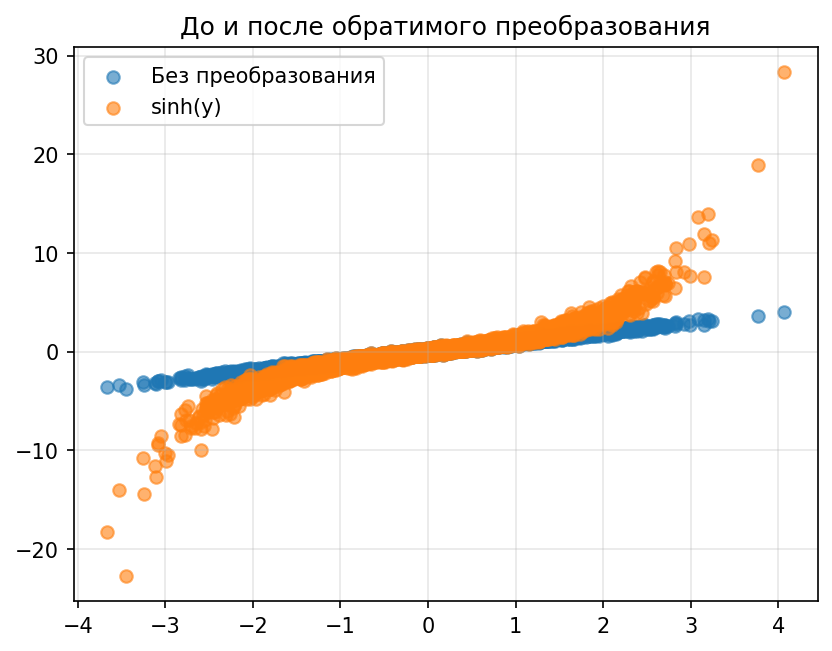
\includegraphics[width=\linewidth]{figs/before_after_transform.png}
  \captionof{figure}{Облако точек до и после $y\mapsto\sinh y$ ($d=1$,
  $\rho=0.99$): форма меняется, информация о связи — нет.}\label{fig:inv}
\end{minipage}\hfill
\begin{minipage}[c]{0.40\linewidth}\centering
  \captionof{table}{Инвариантность к биекциям ($d=3$, $\rho=0.8$).}\label{tab:inv}
  \begin{tabular}{lc}
  \toprule
  Метод & $\hat I$, нат \\
  \midrule
  Истина & 1.532 \\
  \textsc{MINE}$(x,y)$ & 1.511 \\
  \textsc{MINE}$(x,\sinh y)$ & 1.347 \\
  \textsc{MINE}$(x,yA)$ & 1.533 \\
  \bottomrule
  \end{tabular}
\end{minipage}\par\addvspace{6pt}

\sublesson{5.5}{Абляционные эксперименты}

Проведено пять абляций: (1)~архитектура критика, (2)~EMA, (3)~способ получения
отрицательных пар, (4)~размер батча, (5)~ширина сети. Все — при $\rho=0.75$,
$d=10$ (истина $4.133$ нат), и каждое значение — среднее по 5 запускам
(разным сидам), чтобы убрать разброс между ними.

{\fontsize{9}{11}\selectfont\color{muted}Абляции 1--3
(таблицы~\ref{tab:critic}--\ref{tab:neg})}\par\addvspace{3pt}

\textbf{Абляция 1 — архитектура критика.} Линейный критик $T=w\,(x\cdot y)$ не
может воспроизвести квадратичный оптимум \eqref{eq:tstar}, поэтому заметно
занижает оценку: MLP выигрывает около $0.7$ ната (таблица~\ref{tab:critic}).

\textbf{Абляция 2 — EMA.} Отключение EMA меняет оценку примерно на $0.5$ ната,
то есть в пределах разброса между сидами: EMA влияет на стабильность градиента,
а не на систематическое смещение (таблица~\ref{tab:ema}).

\textbf{Абляция 3 — отрицательные пары.} Случайная перестановка и циклический
сдвиг дают практически одинаковый результат (таблица~\ref{tab:neg}).

\par\addvspace{6pt}
\noindent
\begin{minipage}[t]{0.315\linewidth}\centering
  \captionof{table}{Абляция 1 — архитектура критика}\label{tab:critic}
  \begin{tabular}{lc}
  \toprule
  Критик & $\hat I$, нат \\
  \midrule
  Истина & 4.133 \\
  MLP & 3.087 \\
  Линейный & 2.354 \\
  \bottomrule
  \end{tabular}
\end{minipage}\hfill
\begin{minipage}[t]{0.315\linewidth}\centering
  \captionof{table}{Абляция 2 — EMA}\label{tab:ema}
  \begin{tabular}{lc}
  \toprule
  Вариант & $\hat I$, нат \\
  \midrule
  Истина & 4.133 \\
  EMA & 2.999 \\
  Без EMA & 3.533 \\
  \bottomrule
  \end{tabular}
\end{minipage}\hfill
\begin{minipage}[t]{0.315\linewidth}\centering
  \captionof{table}{Абляция 3 — отрицательные пары}\label{tab:neg}
  \begin{tabular}{lc}
  \toprule
  Вариант & $\hat I$, нат \\
  \midrule
  Истина & 4.133 \\
  randperm & 3.061 \\
  shift & 2.930 \\
  \bottomrule
  \end{tabular}
\end{minipage}\par\addvspace{6pt}

{\fontsize{9}{11}\selectfont\color{muted}Абляции 4--5
(рисунок~\ref{fig:batchwidth})}\par\addvspace{3pt}

\textbf{Абляция 4 — размер батча.} С ростом батча оценка растёт: отрицательные
пары берутся из батча, и больший батч точнее аппроксимирует $p(x)p(y)$; при
очень малых батчах критик просто не успевает обучиться за отведённые шаги.

\textbf{Абляция 5 — ширина сети.} Более широкая сеть лучше приближает
оптимальный критик, но после $\approx64$ нейронов оценка выходит на плато: узкое
место — не ёмкость модели, а бюджет обучения (500 шагов при $\eta=10^{-3}$).

\par\addvspace{6pt}
\noindent\begin{minipage}{\linewidth}\centering
  \begin{minipage}[t]{0.47\linewidth}\centering
    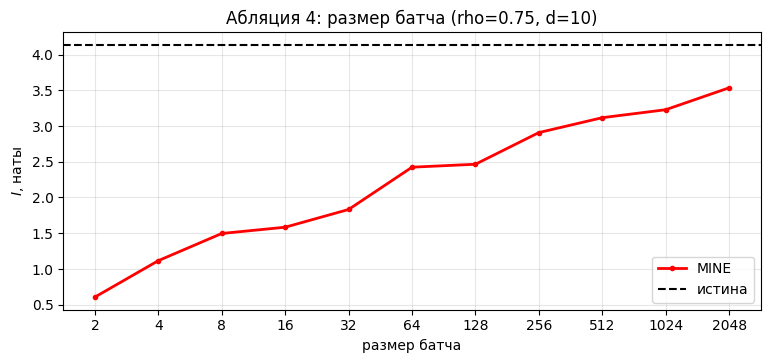
\includegraphics[width=\linewidth]{figs/mine_ablation_batch.png}
  \end{minipage}\hfill
  \begin{minipage}[t]{0.47\linewidth}\centering
    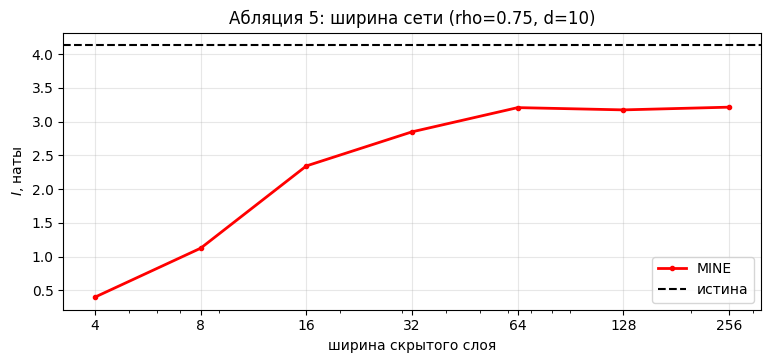
\includegraphics[width=\linewidth]{figs/mine_ablation_width.png}
  \end{minipage}\par
  \captionof{figure}{Абляции 4--5: размер батча (слева) и ширина сети
  (справа). Все точки — среднее по 5 запускам; пунктир — истинное значение
  $4.133$ нат.}\label{fig:batchwidth}
\end{minipage}\par\addvspace{6pt}

Итоги. \textsc{MINE} корректно даёт нижнюю оценку на всём диапазоне
$0.05\ldots19.6$ нат (включая требуемые 2--10), обращается в ноль при
независимости и инвариантен к биекциям.
Качество ограничено ёмкостью критика (линейный критик недобирает $\approx1.8$
ната относительно истины, поле критика это показывает напрямую) и параметрами
обучения (батч, ширина сети). Бейзлайны работоспособны лишь в малой размерности.
Задание требовало
выбрать и реализовать один из двух оценщиков — реализован \textsc{MINE};
верхняя граница \textsc{CLUB} остаётся альтернативой для задач, где ВИ нужно
минимизировать.

% ============================================================================
\heading{Литература}
\noindent\begin{minipage}{\linewidth}
\begin{enumerate}[label={[\arabic*]},leftmargin=2.2em,itemsep=1pt]
  \item Belghazi M. I., Baratin A., Rajeswar S., et al. MINE: Mutual
  Information Neural Estimation // ICML. 2018. arXiv:1801.04062.
  \item Kraskov A., Stögbauer H., Grassberger P. Estimating mutual
  information // Physical Review E. 2004. Vol. 69. 066138.
  \item Cheng P., Hao W., Dai S., et al. CLUB: A Contrastive Log-ratio Upper
  Bound of Mutual Information // ICML. 2020. arXiv:2006.12013.
  \item Cover T. M., Thomas J. A. Elements of Information Theory. 2nd ed.
  Wiley, 2006.
\end{enumerate}
\end{minipage}

\end{document}
